\subsection{Différenciation par les supports (Xavière)}

% BILAN D'ETAPE

%Au départ, je suivais plusieurs pistes de différenciation. En particulier, je souhaitais instaurer un parcours différencié pour mes deux classes principales, selon le modèle présenté par Julia. Ma tutrice ESPÉ m’a fortement conseillé de me limiter à ma classe de 4e, plus difficile à mettre au travail.
%
%J’ai également créé une évaluation à jokers avec ma classe de 4e. Les jokers sont des petits papiers contenant une indication sur l’exercice que je distribue aux élèves en échange d’une pénalité minime sur la note. Cette évaluation a obtenu un franc succès.
%J’ai également commencé le travail d’auto-évaluation avec mes 5e. Ce qu’il manque pour approfondir ce point, c’est créer une métrique adaptée. Pour le moment je n’ai pas de retour quantifiable.
%
%Sur les conseils de Nadine Grapin, je me suis concentrée sur un axe de recherche en particulier, et j’ai choisi l’auto-évaluation. Pour cela, je souhaite m’intéresser aux supports.
%
%Mes classes sont caractérisées par la présence de mauvais lecteurs (des élèves en très grande difficulté en Français, sans toutefois présenter des troubles dys). Il est donc primordial de m’assurer que :
%\begin{enumerate}
%    \item ils se construisent des images mentales correctes et cela ne peut pas toujours passer par une compréhension de la trace écrite. J’ai remarqué, en particulier pour la classe de 5e, que les images mentales dynamiques (nécessitant des manipulations) étaient plus facilement assimilées et restituées par les élèves.
%    \item les consignes données à l’oral sont parfaitement comprises de tous
%\end{enumerate}
%
%De plus, comme je vise l’autonomie des élèves à la fois en classe et hors classe, je dois compléter cette approche par d’autres supports, en particulier des fiches de correction. Pour le moment, je les guide sur la construction de fiches de révision agréables à l’oeil pour que les élèves s’y réfèrent plus volontiers. Je souhaite me tourner progressivement vers des fiches de correction, puis d’auto-correction, avec un guide de construction de fiches créé par les élèves. L’objectif final est de produire des grilles d’auto-évaluation.
%Tout ceci est très expérimental et je ne suis pas encore en capacité de mesurer quantitativement les conséquences de la multiplication des supports

%{\color{red}Tous les passages écrits en rouge dans cette partie sont des remarques destinées à améliorer le contenu, souvent sur la forme, ou sont des réflexions ou des questionnements.}
%
%\subsubsection{Motivations}
%
%{\color{red}Rappels en vrac de ma ligne directrice pour mes expérimentations. À reformuler et à remettre en contexte. Ce sont les conseils donnés par ma tutrice en début d'année que j'ai essayé d'appliquer de mon mieux, à l'exception des vidéos.}
%
%\begin{itemize}
%\item Se renseigner sur la différenciation en axant sur les images mentales ;
%\item diversifier les images mentales (toutes ne fonctionnent pas sur tous les élèves) ;
%\item diversifier les images mentales grâce aux supports :
%\begin{itemize}
%\item cartes mentales (en particulier celles centralisant toutes les façons de répondre à un problème donné, par exemple comment montrer que deux droites sont parallèles) ;
%\item manipulations manuelles/gestuelles ;
%\item utilisation de geogebra par les élèves (et non par moi) ;
%\item vidéos explicatives ;
%\item fiches de méthodologie cartonnées, idéalement faites spontanément par les élèves ;
%\end{itemize}
%\item le but est de fixer par écrit les images mentales.
%\end{itemize}
%
%\paragraph{Quelques détails}
%
%Le but est que \textbf{les élèves créent eux-mêmes leurs outils}. La priorité est aux fiches méthodes, fiches erreur et cartes mentales. Sur les fiches méthodes, lorsque nous voyons une méthode technique en cours, les élèves en font une fiche cartonnée qui leur servira de référence lors des exercices et évaluations. La fiche erreur est construite par l'enseignant sur la base de plusieurs publications des élèves. Je leur donne un bilan récapitulatif des erreurs à éviter. Eux en font une fiche qui complète la fiche méthode. Pour la carte mentale, il est convenu avec ma tutrice que je leur fournisse une base qu'ils complètent.
%
%Je peux aussi leur fournir une carte mentale de résumé de cours, mais comme cela consiste essentiellement en de la recopie du cours, \textbf{ne pas la considérer comme un exercice mathématique} à part entière et ne pas leur donner à compléter.
%
%{\color{red}Faire de tout ce paragraphe un tableau synthétique.}
%
%Le but est de leur permettre de s'emparer, de s'approprier les notions vues en classe et de leur constituer {\color{red}(ou apprendre à constituer)} une banque de ressources qu'ils utiliseront en classe sur exercices ou à la maison pour s'auto-corriger.
%
%Ce travail sera essentiellement \textbf{étudié sur ma classe de 5\up{e}}, mais ceci est proposé sur les deux classes.
%
%Note : ma tutrice ESPÉ m'a conseillé de me limiter aux parcours différenciés aux 4\up{e}. Ceci étant couvert par Julia, je n'en parlerai pas. {\color{red}Retour très intéressant de Claire sur le problème du saucissonnage sur la séquence Pythagore, cela vaut sans doute la peine d'en parler en discussion.}\\
%
%{\color{red} Pour ce qui suit, j'ai le sentiment que cela fait beaucoup trop. J'ai entamé un très gros travail sur la symétrie et j'ai également des scans de copies d'élèves appuyant la nécessité de corriger une mauvaise conception pour les angles alternes-internes. La partie sur le calcul algébrique est sans doute dispensable si je n'en ai pas le temps et je manque de productions d'élèves pour l'étayer. Enfin, la dernière partie sera uniquement axée sur le traitement des erreurs à éviter (ou dans le cas présent, des éléments manquants). J'ai à la fois les productions d'élèves scannées, le fichier regroupant les productions les plus intéressantes et la fiche méthodologique construite par les élèves. Les cartes mentales ont surtout été vues avec les 4e, sur le principe elles reprennent ce qu'on a fait avec les fiches méthodologiques. J'ai encore une séquence à finir et une autre à faire avec mes 5e avant de pouvoir faire des cartes mentales intéressantes portant sur plusieurs séquences.}

%\subsubsection{Symétries : manipulations manuelles et sur geogebra - fiches de méthodologie}
%
%Le but est de montrer comment j'ai ajouté des couches successives pour renforcer les deux images mentales principales en symétrie axiale et symétrie centrale. J'ai toujours un problème avec mon élève italien qui a tendance à effectuer des translations.
%
%\paragraph{Les cocottes en symétrie}
%
%\paragraph{Remplacement progressif par les mains}
%
%\paragraph{Utilisation de GeoGebra en auto-correction}
%
%Lien vers ma séance TICE. Probablement pas aussi développé que le reste.
%
%\paragraph{Fiches de méthodologie}
%
%\paragraph{Retours, productions d'élèves}
%
%Lien vers mon analyse d'évaluation + la toute dernière évaluation faite. Parler de mon élève italien ?
%
%\subsubsection{Angles alternes-internes : comment corriger une potentielle image fausse}
%
%\paragraph{Situation qui a amené les élèves à créer cette image mentale fausse}
%
%Lien vers mini-évaluation + stats rapides sur présence de l'erreur dans les copies.
%
%\paragraph{Utilisation de GeoGebra pour corriger une potentielle image mentale fausse}
%
%\paragraph{Une autre approche : la libellule et la coccinelle}
%
%Très rapide, l'évaluation récente montre que cette image mentale n'est pas très populaire au sein de ma classe, alors qu'elle est très utilisée dans les deux autres classes de 5\up{e} (le timing où elle a été présentée est différent).
%
%\paragraph{Initiation à la démonstration : erreurs et correction par les pairs}
%
%{\color{red} Je ne sais pas si celui-ci a sa place dans ce mémoire, dans la mesure où cela se passe intégralement à l'oral}
%
%\paragraph{Cartes mentales - droites parallèles / calcul d'angles}
%
%Les deux sont envisageables et liées à cette séquence. {\color{red}Je ne sais pas si j'aurai le temps de les amorcer avant la date de rendu du mémoire.}
%
%\subsubsection{Calcul algébrique : deux approches différentes pour toucher un maximum d'élèves}
%
%\paragraph{Nombres relatifs - approche vectorielle}
%
%\paragraph{Nécessité de recourir à une deuxième approche}
%
%\paragraph{Nombres relatifs - approche [nom à définir plus tard]}
%
%\subsubsection{Gestion de données : trouver les erreurs à éviter}
%
%\paragraph{Problème initial et productions d'élèves}
%
%\paragraph{Fiche méthodologique résultante}
%
%\subsubsection{Retours élèves}

\subsubsection{Motivations}

Le but de mon expérimentation était d'amener les élèves de ma classe de 5\up{e} à un niveau suffisant d'autonomie pour créer eux-mêmes leurs propres outils de travail (voir \textsc{Figure \ref{org:xav}} ci-dessous). Pour atteindre ce but, j'ai exploré plusieurs pistes et je souhaite en aborder deux en particulier : le travail effectué autour de la symétrie dans un premier temps et le travail effectué sur les angles alternes-internes dans un deuxième temps.

\begin{figure}[h!]
    \centering
    \tikzstyle{cat1} = [rectangle, rounded corners, minimum width=3cm, minimum height=1cm, text centered, text width=3cm, draw=black, fill=black!0]
\tikzstyle{cat2} = [rectangle, minimum width=3cm, minimum height=1cm, text centered, text width=3cm, draw=black,  fill=black!10]
\tikzstyle{cat3} = [rectangle, minimum width=5cm, text centered, text width=5cm, minimum height=1cm, draw=black,  fill=black!10]

\tikzstyle{arrow} = [thick,->,>=stealth]

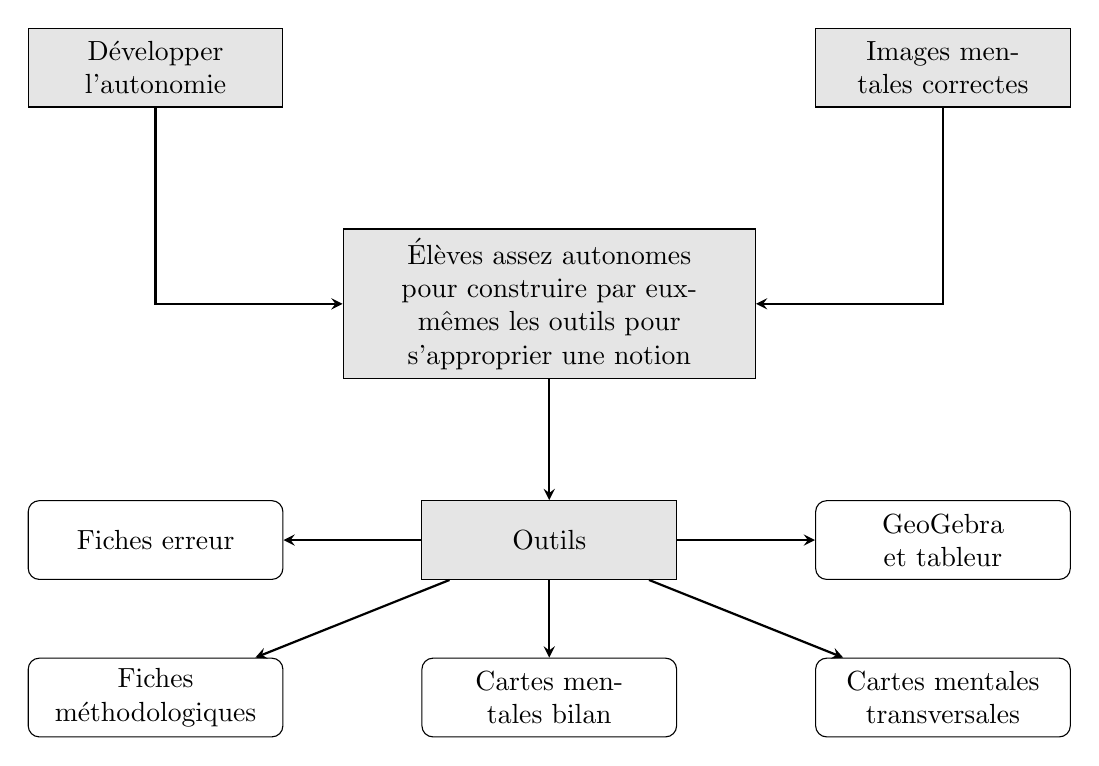
\begin{tikzpicture}[node distance=3cm]
\node (auto) [cat2] {Développer l'autonomie};
\node (img) [cat2, right of=auto, xshift=7cm] {Images mentales correctes};
\node (pb) [cat3, below of=auto, xshift=5cm] {Élèves assez autonomes pour construire par eux-mêmes les outils pour s'approprier une notion};
\node (outils) [cat2, below of=pb] {Outils};
\draw [arrow] (auto) |- (pb);
\draw [arrow] (img) |- (pb);
\draw [arrow] (pb) -- (outils);
\node (fiche1) [cat1, left of=outils, xshift=-2cm] {Fiches erreur};
\node (fiche2) [cat1, below of=outils, xshift=-5cm, yshift=1cm] {Fiches méthodologiques};
\node (carte1) [cat1, below of=outils, yshift=1cm] {Cartes mentales bilan};
\node (geogebra) [cat1, right of=outils, xshift=2cm] {GeoGebra et tableur};
\node (carte2) [cat1, below of=outils, xshift=5cm, yshift=1cm] {Cartes mentales transversales};
\draw [arrow] (outils) -- (fiche1);
\draw [arrow] (outils) -- (fiche2);
\draw [arrow] (outils) -- (geogebra);
\draw [arrow] (outils) -- (carte1);
\draw [arrow] (outils) -- (carte2);
\end{tikzpicture}

    \caption{Organigramme des ressources nécessaires pour amener des élèves à créer leurs propres outils en toute autonomie}
    \label{org:xav}
\end{figure}

\paragraph{Présentation succincte des outils que les élèves sont amenés à utiliser sur l'année}

Voici les quatre types d'outils que je souhaitais expérimenter au cours de mon année de stage.
\begin{itemize}
	\item [\textit{Les fiches méthodologiques :}] accompagnement de cours, elles se présentent sous la forme d'une méthode écrite sur une fiche cartonnée et illustrée selon les goûts des élèves. Les élèves les utilisent lorsqu'ils travaillent sur des exercices ou lors des devoirs avec ma permission.
	\item [\textit{Les fiches erreur :}] ces fiches viennent en complément des fiches méthodologiques. Elles sont utilisées pour aider les élèves à valider ou invalider un résultat. C'est un axe de recherche que je n'ai pas assez développé cette année. J'ai limité mes expérimentations à la présentation d'extraits de copies à mes élèves pour générer des débats. Il en a résulté des fiches méthodologiques au lieu de fiches erreur.
	\item [\textit{Les cartes mentales :}] initialement, si l'on se réfère à la  \textsc{Figure \ref{org:xav}}, il était prévu que je travaille sur deux types de cartes mentales avec les élèves. Le premier type est une carte rappelant les notions importantes du cours, telles qu'on les trouve dans les leçons de cycle 3 ou les manuels de cycle 4. Elle sert de bilan et est surtout utilisée lors des révisions. Les élèves en ont réalisé quelques-unes tout au long de l'année, toujours d'après un modèle établi en commun en classe. \\
	Le second type est une carte mentale transversale, répondant à une question\footnote{Par exemple : « Comment prouver que deux droites sont parallèles ? »} qui peut être traitée à l'aide de procédures issues de plusieurs séquences. J'ai manqué de temps et de recul sur le programme pour mettre ce type de carte mentale en place.
	\item [\textit{L'utilisation des TICE}]\footnote{Technologies de l'Information et de la Communication pour l'Enseignement} \textit{:} les élèves manipulent régulièrement en cours d'année les logiciels utilisés en mathématiques (GeoGebra et les tableurs) pour apprendre à valider un résultat ou une conjecture de manière autonome.
\end{itemize}

Je détaille mon avancement dans l'expérimentation de chacun de ces outils dans la section \ref{sec:retours}.

\subsubsection{Pourquoi la différenciation est importante pour l'autonomie des élèves}

Lorsqu'on cherche à rendre ses élèves autonomes, on se rend vite compte que la différenciation intervient à plusieurs niveaux. Si l'on se réfère à l'organigramme présenté en \textsc{Figure \ref{org:xav}}, la première entrée est la poursuite du développement de l'autonomie, entrepris au cycle 3. J'ai suivi deux axes :
\begin{itemize}
    \item faire acquérir aux élèves le réflexe d'utiliser leurs outils (relire une fiche méthodologique quand on bloque devant un exercice, se référer à la fiche-erreur pour valider un résultat, utiliser les cartes mentales pour réviser...) ;
    \item développer le travail en autonomie en classe, l'objectif au troisième trimestre étant de m'assurer que mes élèves sont en activité un tiers du temps.
\end{itemize}
Concernant le premier point, la différenciation passe essentiellement par une attention particulière aux consignes données et le choix des procédures de résolution (différenciation simultanée \cite{Eduscol}). Ce point ne sera pas détaillé ici.

Concernant le second point, Il faut distinguer deux moments forts du cours lorsqu'on travaille sur les images mentales avec les élèves. Pour rappel, une image mentale est « une représentation d'une information sensitive sans perception d'un stimulus externe » \cite{mimagery}. Cette représentation peut être mémorisée ou imaginée. En mathématiques, les images mentales servent à donner du sens à un concept non perceptible par nos sens.

Dans un premier temps, j'établis avec mes élèves une image mentale (ou plusieurs) à laquelle se référer lorsqu'ils rencontrent un nouveau concept. La différenciation porte sur la variété des supports présentés aux élèves (différenciation successive \cite{Eduscol}).

Dans un deuxième temps, après avoir observé les élèves travailler sur le nouveau concept avec leur(s) image(s) mentale(s), j'entre parfois dans une phase de remédiation : l'image mentale présentée initialement étant mal assimilée ou incomplète. La remédiation passe soit par la présentation d'une autre image mentale, soit par un changement de support pour une même image mentale.

Le travail présenté dans ce mémoire porte sur ces deux temps de fabrication d'une image mentale correcte :
\begin{itemize}
    \item une première sous-partie est consacrée à variété des supports utilisés pour passer d'une perception de la symétrie (axiale et centrale) à une image mentale en variant les sens utilisés ;
    \item une seconde sous-partie est consacrée à la remédiation d'une mauvaise conception des angles alternes-internes.
\end{itemize}

La différenciation intervient également au niveau des outils eux-mêmes : les logiciels nécessitent une phase de prise en main et un de mes axes cette année a été de proposer des exercices différenciés sur support informatique, adaptés à l'aisance des utilisateurs avec les logiciels. J'en parle très brièvement au moment où j'aborde la section consacrée aux symétries.

\subsubsection{Différencier pour acquérir une image mentale : la symétrie}

%Le but est de montrer comment j'ai ajouté des couches successives pour renforcer les deux images mentales principales en symétrie axiale et symétrie centrale. J'ai toujours un problème avec mon élève italien qui a tendance à effectuer des translations.

J'ai commencé à construire la séquence dédiée à la symétrie axiale à l'aide du livre \textit{Des maths ensemble et pour chacun 5\up{e}} \cite{mepcc} (séquence 2, pages 88-103). La première activité présentée utilise des silhouettes de cocottes et les indications à destination de l'enseignant emploient également les cocottes (voir \textsc{Figure \ref{fig:cocottes}} et annexe \ref{annexe:symetrie-act}). J'ai repris cette idée pour mon expérimentation.

\begin{figure}[h!]
    \centering
    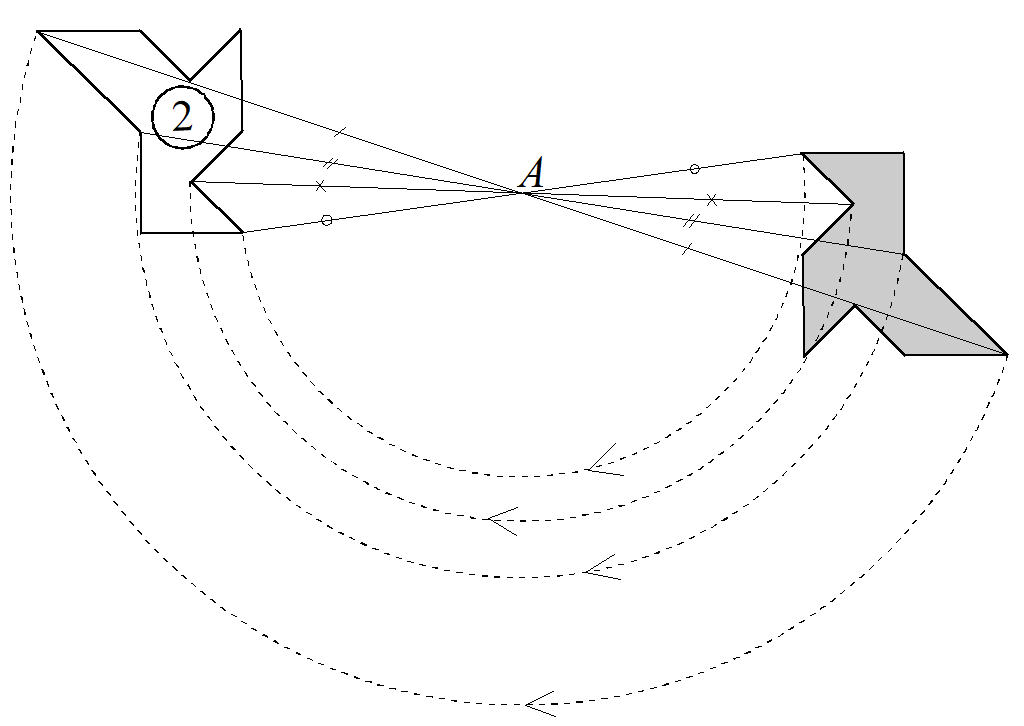
\includegraphics[width=0.6\linewidth]{img/cocottesmepcc.png}
    \caption{Figure accompagnant les explications destinées à l'enseignant et pouvant être photocopiées et distribuées aux élèves}
    \label{fig:cocottes}
\end{figure}

\paragraph{Création d'un outil à manipuler : les cocottes}

En premier lieu, avant de leur donner l'activité du livre qui consistait à classer des couples de cocottes grises et blanches par type de transformation (symétrie axiale, symétrie centrale et translation), j'ai appris aux élèves à créer deux cocottes identiques, excepté un signe distinctif, avec une feuille de papier. Lorsqu'ils ont démarré l'activité, ils superposaient la cocotte blanche sur la cocotte grise et essayaient de trouver quelle manipulation ils faisaient avec les mains pour arriver au résultat présenté sur la feuille d'activité.

Très vite, les élèves ont retrouvé l'image du miroir pour la symétrie axiale et le mouvement rectiligne pour la translation. Ils ont également découvert que leurs cocottes effectuaient un arc de cercle pour la symétrie centrale.

Les cocottes sont pratiques pour deux raisons : premièrement, elles représentent concrètement les figures de l'énoncé. Les élèves n'ont pas à faire un effort d'abstraction supplémentaire pour passer de la manipulation à la situation de l'énoncé. Deuxièmement, elles se glissent toutes dans une pochette et sont facilement transportables. Même si elles sont égarées, elles sont très rapides à fabriquer.

\paragraph{Remplacement progressif par les mains}

La phase de consolidation de l'image mentale s'est faite en deux temps. Tout d'abord, j'ai présenté aux élèves des exercices où les figures n'étaient plus des cocottes, pour qu'elles prennent le statut d'outil. Puis certains élèves ont compris qu'ils effectuaient les mouvements avec les mains qui tenaient les cocottes et ont commencé à faire les manipulations avec les mains seulement.

À ce moment, j'ai moi-même commencé à évoquer les images mentales du miroir et de la rotation avec mes mains sans tenir les cocottes. Le comportement s'est généralisé à l'ensemble de la classe.

\paragraph{Fiches méthodologiques}

Lors du travail sur cette séquence, les élèves ont construits deux fiches méthodologiques pour la symétrie axiale et deux fiches méthodologiques pour la symétrie centrale.

La première fiche détaille la construction de l'axe de symétrie ou du centre de symétrie. Elle a été construite en commun avec la classe après leur avoir fait construire les axes de symétrie et les centres de symétrie à nouveau sur la première activité de la séquence. La fiche résulte du débat généré à la fin de l'exercice et synthétisé par un élève. À ce moment de l'expérimentation, les élèves notaient sur leur feuille des flèches de rotations comme celles que l'on voit sur la \textsc{Figure \ref{fig:cocottes}} pour évoquer l'image mentale qu'ils s'étaient construite.

La seconde fiche détaille la construction du symétrique d'une figure par symétrie axiale ou centrale.

Des exemples sont disponibles dans l'annexe \ref{annexe:symetrie-fiches}.

Ces fiches ont été reproduites sur papier cartonné et étaient utilisées lors des exercices d'entrainement sur la durée ou lors de certains devoirs surveillés.

\paragraph{Utilisation de GeoGebra}

J'ai beaucoup travaillé cette séquence sur la durée et je me suis rendue compte en cours d'année que certains élèves oubliaient l'image mentale s'ils ne travaillaient pas assez régulièrement dessus. Pour les aider, sur un conseil de ma tutrice terrain, Madame Hizembert, j'ai créé une séance en salle informatique pour leur apprendre à utiliser de façon autonome GeoGebra pour s'entrainer chez eux.

Un résumé de la séance est présent dans l'annexe \ref{annexe:symetrie-tice}.

Avec le recul que j'ai à présent et suite à des discussions avec Madame Hizembert, j'aurais pu utiliser davantage GeoGebra pour renforcer les images mentales des élèves. La séance informatique est intervenue trop tard dans l'année. J'ai également découvert que le manuel \textit{Des maths ensemble et pour chacun 5\up{e}} s'accompagnait d'un site\footnote{Site compagnon : \url{http://edition.crdp-nantes.fr/?id=maths-ensemble-et-pour-chacun}} permettant de télécharger des ressources qui permettent de visualiser l'image mentale de la rotation avec GeoGebra.

\subsubsection{Remédier à une mauvaise conception : les angles alternes-internes}

Lorsque j'ai introduit les angles alternes-internes aux élèves, j'ai très rapidement réutilisé les propriétés de conservation de la symétrie centrale (travail sur la durée), couplée à une conjecture visualisée à l'aide de GeoGebra, alors que la définition d'angles alternes-internes n'avait pas été vue. En conséquence, sur une évaluation diagnostique qui a suivi peu après, j'ai constaté que pour beaucoup d'élèves (voir annexe \ref{annexe:angles-prod1}), deux angles alternes internes étaient \textbf{toujours} définis par deux droites \textbf{parallèles} et une sécante. J'ai aussi pu constater que pour un grand nombre d'élèves, il n'existe qu'une paire d'angles alternes-internes, la paire d'angles aigus ou au contraire la paire d'angles obtus.

J'ai choisi deux axes de remédiation. Tout d'abord, j'ai travaillé sur des exercices très progressifs (sur le principe du parcours différencié). Puis j'ai présenté une nouvelle image mentale aux élèves qui avaient encore du mal à transposer les mots de la définition des angles alternes-internes à une application concrète.

\paragraph{Exercices progressifs}

Les trois fiches d'exercice sont disponibles dans l'annexe \ref{annexe:angles-fiches}

La première fiche d'exercices ne mentionne pas le statut des droites définissant les angles alternes-internes. Le but était de simplement vérifier si la définition correspondaient à ce qu'ils voyaient (présence d'angles alternes-internes, correspondants, alternes-externes, opposés par le sommet et le cas particulier des angles alternes-internes où l'un des angles est un angle droit).

Puis j'ai rétabli que la mention de droites parallèles n'intervient nullement dans la définition mais est prépondérante dans la propriété \textit{« Deux droites parallèles coupées par une droite sécante déterminent des angles alternes-internes de même mesure »} (et sa réciproque). Pour renforcer cette idée, j'ai présenté une nouvelle feuille d'exercices contenant des schémas où toutes les situations montrent des droites parallèles, mais où la mention de droites parallèles est parfois absente (l'un des objectifs étant de travailler sur le passage progressif à la géométrie abstraite).

La troisième feuille d'exercices a été distribuée une fois que les problèmes relevés ont été corrigés et présente des situations de plus en plus complexes.

J'avais dans l'idée d'appliquer le principe des parcours différenciés mais l'exécution a été maladroite. La fiche 3 est celle où le principe apparait le plus clairement : seules les situations A, B et C étaient à traiter, les autres étaient réservées aux élèves plus avancés (différenciation simultanée \cite{Eduscol}).

\paragraph{Remédiation par l'acquisition d'une nouvelle image mentale}

Suite à tout ce travail, j'ai constaté que certains élèves avaient encore des difficultés à visualiser les paires d'angles alternes-internes et plus particulièrement le concept derrière le mot alterne. Je leur ai donc conté une histoire venant de ma tutrice terrain, madame Hizembert : « Deux insectes, une coccinelle et une libellule ont rendez-vous d'un coté du pont au-dessus de la rivière. Problème, elles sont chacune d'un coté différent du pont. Elles ne se rencontreront jamais. »

Ce petit texte a été accompagné d'un dessin que quelques élèves se sont appropriés (voir quelques copies d'élèves dans l'annexe \ref{annexe:angles-prod2}). À ma surprise, après avoir présenté cette histoire à toute la classe et après un rapide sondage, il s'est avéré que ceux pour qui la notion était acquise n'appréciaient pas du tout cette histoire.

\subsubsection{Autres expérimentations}

De la même manière que j'ai proposé une nouvelle image mentale pour les angles alternes-internes, j'ai également proposé deux approches lorsque nous avons abordé la séquence de la somme de deux nombres relatifs. J'ai aussi brièvement tenté une évaluation différenciée et j'ai fait travailler mes élèves sur l'auto-évaluation.

Je n'ai pas assez exploité les fiches erreur au cours de cette année. J'ai brièvement utilisé des travaux d'élèves pour travailler sur la mise en forme des données. Bien quel les élèves ont travaillé sur la détection d'erreurs, ils ont abouti à la construction d'une fiche méthodologique. Par la suite, j'ai employé à nouveau les ressources des livres pour les enseignants pour fournir des fiches erreur\footnote{\textit{Des maths ensemble et pour chacun 5\up{e}} \cite{mepcc} (séquence 13, page 245)} sur deux séquences portant sur la construction de triangles.

J'ai également développé avec ma classe de 4\up{e} des évaluations à joker, qui sont une autre forme de différenciation. Le principe ayant rencontré un certain succès, tant au niveau de la motivation des élèves qu'au niveau de l'évaluation des acquis, je l'ai également appliqué à ma classe de 5\up{e}.

Ces dispositifs mériteraient un plus gros développement (voir section \ref{sec:retours}). La soutenance orale sera l'occasion d'y revenir.

\subsubsection{Retours des élèves}

Cette partie de l'expérimentation n'est pas encore menée. J'aurais aimé soumettre un questionnaire à mes élèves portant sur la fréquence à laquelle ils emploient leurs outils, dans quelles circonstances, l'aisance avec laquelle ils créeraient seuls leurs outils, l'utilisation de GeoGebra et du tableur chez soi...

Le planning propre à mon collège me laisse peu de marge de manœuvre pour leur soumettre le questionnaire avant la soutenance orale, mais si j'en ai l'occasion, l'aimerais également aborder ce point lors de la soutenance.
